
\documentclass[11pt,a4paper]{article}
\usepackage[hyperref]{naaclhlt2018}
%\usepackage[nohyperref]{naaclhlt2018}
\usepackage{times}
\usepackage{latexsym}

% both ICLR and NAACL
\usepackage{url}
\usepackage{multirow}
\usepackage{graphicx}
\usepackage{amsmath}
\usepackage{array}



\title{Deep contextualized word representations}

% Authors must not appear in the submitted version. They should be hidden
% as long as the \iclrfinalcopy macro remains commented out below.
% Non-anonymous submissions will be rejected without review.

% FOR NAACL
%\setlength\titlebox{5cm}
% You can expand the titlebox if you need extra space
% to show all the authors. Please do not make the titlebox
% smaller than 5cm (the original size); we will check this
% in the camera-ready version and ask you to change it back.


\author{Matthew E. Peters$^\dagger$, Mark Neumann$^\dagger$, Mohit Iyyer$^\dagger$, Matt Gardner$^\dagger$, \\
\texttt{\{matthewp,markn,mohiti,mattg\}@allenai.org} \\
\AND
Christopher Clark$^*$, Kenton Lee$^*$, Luke Zettlemoyer$^{\dagger*}$ \\
\texttt{\{csquared,kentonl,lsz\}@cs.washington.edu} \\
%\AND
\\ $^\dagger$Allen Institute for Artificial Intelligence \\
$^*$Paul G. Allen School of Computer Science \& Engineering, University of Washington
}

% The \author macro works with any number of authors. There are two commands
% used to separate the names and addresses of multiple authors: \And and \AND.
%
% Using \And between authors leaves it to \LaTeX{} to determine where to break
% the lines. Using \AND forces a linebreak at that point. So, if \LaTeX{}
% puts 3 of 4 authors names on the first line, and the last on the second
% line, try using \AND instead of \And before the third author name.

\newcommand{\fix}{\marginpar{FIX}}
\newcommand{\new}{\marginpar{NEW}}
\newcommand{\ELMO}{ELMo}
% use like \tinysection{Word sense disambiguation}
\newcommand{\tinysection}[1]{\textbf{#1}}
%\newcommand{\tinysection}[1]{\textbf{#1} \\}

% to add comments inline
\newcommand\mpcomment[1]{\textcolor{blue}{\textbf{[#1] --\textsc{MP}}}}
\newcommand\mgcomment[1]{\textcolor{blue}{\textbf{[#1] --\textsc{MG}}}}
\newcommand\micomment[1]{\textcolor{red}{\textbf{[#1] --\textsc{MI}}}}

%\iclrfinalcopy % Uncomment for camera-ready version, but NOT for submission. ICLR

\aclfinalcopy % Uncomment this line for the final submission
%\def\aclpaperid{5} %  Enter the acl Paper ID here

\begin{document}


\maketitle

\begin{abstract}
We introduce a new type of {\em deep contextualized} word representation that models both (1) complex characteristics of word use (e.g., syntax and semantics), and (2) how these uses vary across linguistic
contexts (i.e., to model polysemy).
%how complex aspects of word use (e.g. syntax and semantics) vary with the linguistic context in which the word is used (i.e. to model polysemy).
Our word vectors are learned functions of the internal states of a deep bidirectional language model (biLM), which is pre-trained on a large text corpus.
%Our word vectors are linear functions of the internal states of a deep bi-directional language model, which is pretrained on a large text corpus.
We show that these representations can be easily added to existing models and significantly improve the state of the art across six challenging NLP problems, including question answering, textual entailment and sentiment analysis.
%We show that these \ELMO\  (Embeddings from Language Models) representations can be easily added to existing models for six challenging NLP problems, including sentiment analysis and question answering, and that they significantly improve state-of-the-art performance levels in every case.
We also present an analysis showing that exposing the deep internals of the pre-trained network is crucial, allowing downstream models to mix different types of semi-supervision signals.
%to explain why these representations work so well in practice, which highlights the benefits of exposing the internal states of the pretrained deep networks. 



%We present a general method to add context dependent word representations from a pre-trained, large scale bidirectional language model (biLM) to any supervised NLP architecture.
%By allowing the supervised model to learn a weighted combination of all biLM layers, it can preferentially re-use the different types of information represented at each biLM layer in a task specific way.
%This approach works well in practice, establishing
%We establish six new state-of-the-art results on a diverse set of benchmark NLP tasks for textual entailment, question answering, coreference resolution, semantic role labeling, named entity extraction, and sentiment classification, in all cases significantly improving overall system performance.
%We attribute the improved performance on supervised tasks to the biLM's ability to disambiguate word sense and learn basic elements of syntax.
%Finally, in every considered case, the biLM outperforms contextual embeddings produced by a machine translation system.

\end{abstract}

\section{Introduction}
Pre-trained word representations~\citep{word2vec,Pennington2014GloveGV} are a key component in many neural language understanding models. 
However, learning high quality representations can be challenging.
They should ideally model both (1) complex characteristics of word use (e.g., syntax and semantics), and (2) how these uses vary across linguistic
contexts (i.e., to model polysemy).
In this paper, we introduce a new type of {\em deep contextualized} word representation that directly addresses both challenges, can be easily integrated into existing models, and significantly improves the state of the art in every considered case across a range of challenging language understanding problems.
%In this paper, we introduce a new type of {\em deep contextualized} word representation that directly addresses both challenges, can be easily integrated into existing models, and significantly improves the state of the art on a range of challenging language understanding problems.


Our representations differ from traditional word type embeddings in that each token is assigned a representation that is a function of the entire input sentence. We use vectors derived from a bidirectional LSTM that is trained with a coupled language model (LM) objective on a large text corpus. For this reason, we call them \ELMO\ (Embeddings from Language Models) representations. Unlike previous approaches for learning contextualized word vectors~\citep{Peters2017SemisupervisedST,McCann2017LearnedIT}, \ELMO\ representations are deep, in the sense that they are a function of all of the internal layers of the biLM. More specifically, we learn a linear combination of the vectors stacked above each input word for each end task, which markedly improves performance over just using the top LSTM layer.

Combining the internal states in this manner allows for very rich word representations.  Using intrinsic evaluations, we show that the higher-level LSTM states capture context-dependent aspects of word meaning (e.g., they can be used without modification to perform well on supervised word sense disambiguation tasks) while lower-level states model aspects of syntax (e.g., they can be used to do part-of-speech tagging). Simultaneously exposing all of these signals is highly beneficial, allowing the learned models select the types of semi-supervision that are most useful for each end task. 

Extensive experiments demonstrate that \ELMO\ representations work extremely well in practice.
%We first show that they can be easily added to existing models for six diverse and challenging language understanding problems, including sentiment analysis and question answering.
We first show that they can be easily added to existing models for six diverse and challenging language understanding problems, including textual entailment, question answering and sentiment analysis.
The addition of \ELMO\ representations alone significantly improves the state of the art in every case, including up to 20\% relative error reductions.
For tasks where direct comparisons are possible, \ELMO\ outperforms CoVe~\citep{McCann2017LearnedIT}, which computes contextualized representations using a neural machine translation encoder.
Finally, an analysis of both \ELMO{} and CoVe reveals that deep representations outperform those derived from just the top layer of an LSTM.
%Finally, an analysis of ELMo reveals that deep representations are generally useful (it never hurts to expose the internals of the pretrained model), and the LM supervision in \ELMO\ representations consistently provides the strongest performance.\micomment{where exactly in the paper is the LM supervision claim demonstrated? seems not important enough to mention in intro}
Our trained models and code are publicly available, and we expect that ELMo will provide similar gains for many other NLP problems.\footnote{\url{http://allennlp.org/elmo}}

%Largely driven by empirical performance as we will see in detail later, our focus is on computing deep contextualized representations from language models. We introduce \ELMO\ (Embeddings from Language Models) representations that are computed from two large-scale pre-trained deep LSTM language models, one the runs left to right over an input sentence and one that is trained for the reverse direction. Whereas previous contextualized word representations~\citep{Peters2017SemisupervisedST} would only use the output vectors (top layer) from these models, we expose the internal representations at every network layer. The resulting \ELMO\ representations for each input word are simply a linear combination of these state vectors, with coefficients that are learned for each end task. 
 



%--------


%\begin{enumerate}
%\item context representations improve downstream task compared to context independent word vectors
%\item biLMs use lots of unlabeled data to capture many different types of context and learn a rich layered set of representations.
%\item biLMs implicitly learn to do WSD and understand syntax. They separate the information across layers with semantic WSD at top layers and syntax at lower layer
%\item using all layers improves supervised NLP task performance over just top layer -- this is generally true for multiple objective functions including LM and MT
%\item language modeling appears to be better then machine translation for learning representations 
%\end{enumerate}

%Due to their ability to capture syntactic and semantic information of words from large
%scale unlabeled text, pre-trained word embeddings \citep{word2vec,Pennington2014GloveGV} are a standard component in most
%current state-of-the-art NLP architectures (TODO: add refs).
%However, for most NLP tasks, it is important to represent the meaning of
%a word in its context, in addition to the context independent representations of word vectors.
%This is especially important for polysemous words or ones that do not have readily available pre-trained vectors.
%Accordingly, most NLP architectures
%encode contextual information, typically with either a recurrent neural network (RNN)
%or convolutional neural network (CNN) (TODO: add refs) before adding task specific output or attention layers.

%In this paper, we present a general method to improve the performance of supervised NLP systems with context dependent word representations from a character based recurrent bidirectional language model \citep{Peters2017SemisupervisedST}.
%In doing so, we overcome two of the chief limitations of word embeddings -- their context independence and lack of support for out-of-vocabulary tokens.
%As the input token representation is fully character based, the biLM also gracefully handles out-of-vocabulary tokens.
%The method is simple and generally applicable to any supervised NLP architecture including RNNs and CNNS.
%Despite it's simplicity, \ELMO{} (Embeddings from Language Models) improves performance substantially on a wide range of NLP tasks including
%classification, semantic role labeling (SRL), sequence tagging, coreference resolution and end-to-end question answering.

%Previous work has shown that for multi-task training introducing supervision of lower level tasks such as part-of-speech (POS) tagging at lower layers
%improves overall performance of higher level tasks such as dependency parsing \citep{joint-many-iclr07} or CCG super tagging \citep{Sgaard2016DeepML} in a deep LSTM architecture.
%In a RNN based encoder-decoder machine translation system, \citet{Belinkov2017WhatDN} showed that the representations learned at the first layer
%in a 2-layer LSTM encoder are better at predicting POS tags then second layer, despite higher BLEU scores in the 2-layer vs. 1-layer system.
%This suggests that each layer of a deep biLM may represent different information, and allowing access to all levels in a supervised system will improve overall performance on downstream tasks.
%Indeed, our best performing systems allow the supervised model to learn a task specific combination of all biLM layers.
%An empirical analysis of the biLM layers confirms that the lower layer representations are better for a syntactic POS tagging task,
%while the top layer is superior for a semantic fine grained word sense disambiguation task.


\section{Related work}

%\micomment{need to discuss word sense embedding papers}

Due to their ability to capture syntactic and semantic information of words from large scale unlabeled text, pretrained word vectors \citep{Turian2010WordRA,word2vec,Pennington2014GloveGV} are a standard component of most state-of-the-art NLP architectures, including for question answering \citep{liu2017stochastic}, textual entailment \citep{Chen2017EnhancedLF} and semantic role labeling \citep{He2017DeepSR}.
However, these approaches for learning word vectors only allow a single context-independent representation for each word.
%Another line of research focuses on global methods for learning sentence and document encoders from unlabeled data \cite[e.g., ][]
%{Le2014DistributedRO,Kiros2015SkipThoughtV,Hill2016LearningDR,Conneau2017SupervisedLO}, where the goal is to build one representation for an entire text sequence.
%It differs in that we learn a contextual representation for each token whereas these methods learn one encoder for an entire text sequence.
%, in addition to a single representation of each word's context that is either discarded after training (in the case of \texttt{word2vec}) or averaged with the word representation (in the case of GLoVe).
%In contrast, as we will see Section~\ref{sec:elmo}, \ELMO\ representations are associated with individual words, but also encode the larger context in which they appear.

Previously proposed methods overcome some of the shortcomings of traditional word vectors by either enriching them with subword information \citep[e.g., ][]{Wieting2016CharagramEW,Bojanowski2017EnrichingWV} or learning separate vectors for each word sense \citep[e.g., ][]{Neelakantan2014EfficientNE}.
Our approach also benefits from subword units through the use of character convolutions, and we seamlessly incorporate multi-sense information into downstream tasks without explicitly training to predict predefined sense classes.
%use bidirectional language models (biLMs) that depend on both context independent word characteristics (e.g. morphology through the use of character convolutions) and the entire sentential context.


Other recent work has also focused on learning context-dependent representations.
\texttt{context2vec} \citep{Melamud2016context2vecLG} uses a bidirectional Long Short Term Memory \citep[LSTM; ][]{LSTM:Hochreiter1997} to encode the context around a pivot word. Other approaches for learning contextual embeddings include the pivot word itself in the representation and are computed with the encoder of either a supervised neural machine translation (MT) system \citep[CoVe; ][]{McCann2017LearnedIT} or an unsupervised language model \citep{Peters2017SemisupervisedST}.
Both of these approaches benefit from large datasets, although the MT approach is limited by the size of parallel corpora.
%whereas the biLM approach limited only by current hardware capabilities.
In this paper, we take full advantage of access to plentiful monolingual data, and train our biLM 
%with significantly larger representations then CoVe 
on a corpus with approximately 30 million sentences \citep{Chelba2014OneBW}.
We also generalize these approaches to deep contextual representations, which we show work well across a broad range of diverse NLP tasks. 

Previous work has also shown that different layers of deep biRNNs encode different types of information.
%necessary for modeling complex end-to-end tasks.
For example, introducing multi-task syntactic supervision (e.g., part-of-speech tags) at the lower levels of a deep LSTM can improve overall performance of higher level tasks such as dependency parsing \citep{joint-many-iclr07} or CCG super tagging \citep{Sgaard2016DeepML}.
In an RNN-based encoder-decoder machine translation system, \citet{Belinkov2017WhatDN} showed that the representations learned at the first layer
in a 2-layer LSTM encoder are better at predicting POS tags then second layer.
Finally, the top layer of an LSTM for encoding word context~\citep{Melamud2016context2vecLG} has been shown to learn representations of word sense. We show that similar signals are also induced by the modified language model objective of our \ELMO\ representations, and it can be very beneficial to learn models for downstream tasks that mix these different types of semi-supervision. 

%allow the supervised model to learn a task specific combination of all biLM layers. 
%, despite higher BLEU scores in the 2-layer vs. 1-layer system.
%An empirical analysis confirms the biLM layers have similar behavior
%-- the lower layer representations are better for a syntactic POS tagging task, while the top layer is superior for a semantic fine grained word sense disambiguation (WSD) task --
%suggesting that allowing access to all layers of the biLM in a supervised system will improve overall performance on downstream tasks.
%Indeed, our best performing systems allow the supervised model to learn a task specific combination of all biLM layers. 

%Similar to computer vision where representations from deep CNNs pretrained on ImageNet are fine tuned for other tasks \citep{alexnet,Shelhamer2015FullyCN},
\citet{Dai2015SemisupervisedSL} and \citet{Ramachandran2017ImproveSeq2SeqLMGal2016ATG} pretrain encoder-decoder pairs
using language models and sequence autoencoders 
and then fine tune with task specific supervision.
In contrast, after pretraining the biLM with unlabeled data, we fix the weights and add additional task-specific model capacity, allowing us to leverage large, rich and universal biLM representations for cases where downstream training data size dictates a smaller supervised model.

%\begin{itemize}
%\item Connections to representation learning in computer vision, except use unsupervised learning instead of large scale supervised data.
%\item lack of large scale supervised datasets in NLP
%\item Alternate approach is machine translation, will compare results later
%\end{itemize}


%\begin{itemize}
%\item Representation learning in NLP has long history.
%\item word representations
%\item sentence representations -- skip thought, fast sent, EMNLP paper for sentence embeddings, sentiment neuron
%\item CoVe
%\item Recent work with biLMs - Peters et al, recent NER paper using biLMs. Mention that Peters et al showed biLM > forward LM, and highlighted importance of large scale training for LM. So restrict to just large scale biLMs in this paper.
%\item Initializing supervised models with LM \citet{Ramachandran2017ImproveSeq2SeqLMGal2016ATG}, except they fine tuned on very large supervised tasks, and have align desired supervised model size with LM size.  Also \citet{Dai2015SemisupervisedSL}
%\item context2vec
%\end{itemize}


\section{\ELMO: Embeddings from Language Models}
\label{sec:elmo}

Unlike most widely used word embeddings~\citep{Pennington2014GloveGV}, \ELMO{} word representations are functions of the entire input sentence, as described in this section. They are computed on top of two-layer biLMs with character convolutions (Sec.~\ref{sec:bilm_def}), as a linear function of the internal network states (Sec.~\ref{sec:compute_elmo}). This setup allows us to do semi-supervised learning, where the biLM is pretrained at a large scale (Sec.~\ref{sec:pretrainedLMs}) and easily incorporated into a wide range of existing neural NLP architectures (Sec.~\ref{sec:using_bilm}). 

%This section details how we compute \ELMO{} representations and use them to improve NLP models.We first present our biLM approach (Sec.~\ref{sec:bilm_def}) and then show how \ELMO\ representations are computed on top of them (Sec.~\ref{sec:compute_elmo}). We also describe how to add \ELMO{} to existing neural NLP architectures (Sec.~\ref{sec:using_bilm}), and the details of how the biLM is pretrained (Sec.~\ref{sec:pretrainedLMs}).

%%%%%%%%%%% BIDIRECTIONAL LANGUAGE MODELS
\subsection{Bidirectional language models}
\label{sec:bilm_def}
Given a sequence of $N$ tokens, $(t_1, t_2, ..., t_N)$, a forward language model computes the probability of the sequence
by modeling the probability of token $t_k$ given the history $(t_1, ..., t_{k-1})$:
\[
p(t_1, t_2, \ldots, t_N) = \prod_{k=1}^N p({t_k} \mid t_1, t_2, \ldots, t_{k-1}).
\]
Recent state-of-the-art neural language models \citep{Jzefowicz2016ExploringTL,Melis2017OnTS,Merity2017RegularizingAO}
compute a context-independent token representation $\mathbf{x}^{LM}_{k}$
(via token embeddings or a CNN over characters) then pass it through $L$ layers of forward LSTMs.
At each position $k$, each LSTM layer outputs a context-dependent representation $\overrightarrow{\mathbf{h}}^{LM}_{k,j}$ where $j=1, \ldots, L$.
The top layer LSTM output, $\overrightarrow{\mathbf{h}}^{LM}_{k,L}$, is used to predict the next token $t_{k+1}$ with a Softmax layer.


A backward LM is similar to a forward LM, except it runs over the sequence in reverse, predicting the previous token given the future context: 
\[
p(t_1, t_2, \ldots, t_N) = \prod_{k=1}^N p(t_k \mid t_{k+1}, t_{k+2}, \ldots, t_N).
\]
It can be implemented in an analogous way to a forward LM, with each backward LSTM layer $j$ in a $L$ layer deep model producing
representations $\overleftarrow{\mathbf{h}}^{LM}_{k,j}$ of $t_k$ given $(t_{k+1}, \ldots, t_N)$.

A biLM combines both a forward and backward LM.  Our formulation jointly maximizes the log likelihood of the forward and backward directions:
\[
\begin{split}
% split added to break eqn for NAACL.  & and \right., \left. also added
\sum_{k=1}^N \left( \right. & \log p({t_k} \mid t_1, \ldots, t_{k-1}; \Theta_x, \overrightarrow{\Theta}_{LSTM}, \Theta_s) \\
+  & \log p({t_k} \mid t_{k+1}, \ldots, t_{N}; \Theta_x, \overleftarrow{\Theta}_{LSTM}, \Theta_s)
\left. \right).
\end{split}
\]
We tie the parameters for both the token representation ($\Theta_x$) and Softmax layer ($\Theta_s$) in the forward and backward
direction while maintaining separate parameters for the LSTMs in each direction.  Overall, this formulation is similar to the approach
of \citet{Peters2017SemisupervisedST}, with the exception that we share some weights between directions instead of using completely independent parameters. In the next section, we depart from previous work by introducing a new approach for learning word representations that are a linear combination of the biLM layers.

%%%%%%%%%%%%%%  COMPUTING ELMO
\subsection{\ELMO{}}
\label{sec:compute_elmo}
\ELMO{} is a task specific combination of the intermediate layer representations in the biLM.
For each token $t_k$, a $L$-layer biLM computes a set of $2L + 1$ representations
%\[  % ICLR
%R_k = \{\mathbf{x}^{LM}_{k}, \overrightarrow{\mathbf{h}}^{LM}_{k,j}, \overleftarrow{\mathbf{h}}^{LM}_{k,j} %\ |\  j = 1, \ldots, L \} =
%    \{\mathbf{h}^{LM}_{k,j}\ | \ j=0, \ldots, L\},
%\]
\begin{eqnarray*}
R_k & =&  \{\mathbf{x}^{LM}_{k}, \overrightarrow{\mathbf{h}}^{LM}_{k,j}, \overleftarrow{\mathbf{h}}^{LM}_{k,j} \ |\  j =1, \ldots, L \} \\
 & = & \{\mathbf{h}^{LM}_{k,j}\ | \ j=0, \ldots, L\},
\end{eqnarray*}
where $\mathbf{h}^{LM}_{k,0}$ is the token layer and $\mathbf{h}^{LM}_{k,j} = [\overrightarrow{\mathbf{h}}^{LM}_{k,j}; \overleftarrow{\mathbf{h}}^{LM}_{k,j}]$, for each biLSTM layer.
%These are the context independent token representation and the hidden states of each directional LSTM at each layer.

For inclusion in a downstream model, \ELMO{} collapses all layers in $R$ into a single vector, $\mathbf{ELMo}_k = E(R_k; \mathbf{\Theta}_e)$.
In the simplest case, \ELMO{} just selects the top layer, $E(R_k) = \mathbf{h}^{LM}_{k,L}$, as in TagLM \citep{Peters2017SemisupervisedST} and CoVe \citep{McCann2017LearnedIT}.
%Across the tasks considered, the best performance was achieved by weighting all biLM layers with a trainable scalar weights:
%\begin{equation}
%E(R_k; \mathbf{w}, \gamma) = \gamma \sum_{j=0}^L s_j \left(\frac{\mathbf{h}^{LM, j}_k - \mu_j}{\sigma_j}\right). \label{eqn:weight_func}
%\end{equation}
%Considering that the activations of each biLM layer have a different distribution, we apply layer normalization to each biLM layer \citep{Ba2016LayerN} before weighting with the softmax normalized learned scalar weights $\mathbf{s} = Softmax(\mathbf{w})$.
More generally, we compute a task specific weighting of all biLM layers:
\begin{equation}
\mathbf{ELMo}^{task}_k = E(R_k; \Theta^{task}) = \gamma^{task} \sum_{j=0}^L s^{task}_j \mathbf{h}^{LM}_{k,j}. \label{eqn:weight_func}
\end{equation}
%For example, our SQuAD model (see Sec. \ref{sec:results}) includes \ELMO{} representations at both the input and output of the task specific RNN.
In (\ref{eqn:weight_func}), $\mathbf{s}^{task}$ are softmax-normalized weights and the scalar parameter $\gamma^{task}$ allows the task model to scale the entire \ELMO{} vector.  $\gamma$ is of practical importance to aid the optimization process (see supplemental material for details).
%Across the tasks considered, the best performance was achieved by weighting all biLM layers with softmax-normalized learned scalar weights $\mathbf{s} = Softmax(\mathbf{w})$:
%\begin{equation}
%E(R_k; \mathbf{w}, \gamma) = \gamma \sum_{j=0}^L s_j \mathbf{h}^{LM, j}_k. \label{eqn:weight_func}
%\end{equation}
%The scalar parameter $\gamma$ allows the task model to scale the entire \ELMO{} vector and is of practical importance to aid the optimization process (see the Appendix for details).
Considering that the activations of each biLM layer have a different distribution, in some cases it also helped to apply layer normalization \citep{Ba2016LayerN} to each biLM layer before weighting.


%%%%%%%%%%%%%%%%%%%%% USING biLMS IN SUPERVISED NLP TASKS
\subsection{Using biLMs for supervised NLP tasks}
\label{sec:using_bilm}
Given a pre-trained biLM and a supervised architecture for a target NLP task, it is a simple process to use the biLM to improve the task model.
We simply run the biLM and record all of the layer representations for each word.  Then, we let the end task model learn a linear combination of these representations, as described below. 

%We simply run the biLM, record all of the vectors it predicts stacked above each word, and let the end task model learn a linear combination of them to predict each word representation, as described in detail below. All of the architectures considered in this paper use RNNs, although the method is equally applicable to CNNs or feed forward networks.

First consider the lowest layers of the supervised model without the biLM.
%Most RNN based NLP models (including every model in this paper) share a common architecture at the lowest layers, allowing us to add \ELMO{} in a consistent, unified manner.
%Given a sequence of tokens $(t_1, \ldots, t_N)$, it is standard to form a context-independent token representation $\mathbf{x}_k$ for each token position using pre-trained word embeddings and optionally character-based representations. % (typically from a CNN).
Most supervised NLP models share a common architecture at the lowest layers, allowing us to add \ELMO{} in a consistent, unified manner.
Given a sequence of tokens $(t_1, \ldots, t_N)$, it is standard to form a context-independent token representation $\mathbf{x}_k$ for each token position using pre-trained word embeddings and optionally character-based representations.
Then, the model forms a context-sensitive representation
$\mathbf{h}_k$, typically using either bidirectional RNNs, CNNs, or feed forward networks.

%Then, one or more layers of bidirectional RNNs compute a context-sensitive representation $\mathbf{h}_k$ for each token position $k$, where $\mathbf{h}_k$ is the concatenation $[\overrightarrow{\mathbf{h}}_{k}; \overleftarrow{\mathbf{h}}_{k}]$ of the forward and backward RNNs.
%Then, one or more layers of bidirectional RNNs compute a context-sensitive representation, $\mathbf{h}_k = [\overrightarrow{\mathbf{h}}_{k}; \overleftarrow{\mathbf{h}}_{k}]$, the concatenation of the forward and backward RNNs.

%$\mathbf{h}_k = [\overrightarrow{\mathbf{h}}_{k}; \overleftarrow{\mathbf{h}}_{k}]$, the concatenation of the hidden states from the forward ($\overrightarrow{\mathbf{h}}_{k}$) and backward ($\overleftarrow{\mathbf{h}}_{k}$) RNNs.

To add \ELMO{} to the supervised model, we first freeze the weights of the biLM and then concatenate the \ELMO{} vector $\mathbf{\ELMO}^{task}_k$ with $\mathbf{x}_k$ and pass the \ELMO{} enhanced representation $[\mathbf{x}_k; \mathbf{\ELMO}^{task}_k]$ into the task RNN.
%To add the biLM to the supervised model, we simply include \ELMO\ as additional input to the task RNN by replacing $\mathbf{x}_k$ with $[\mathbf{x}_k; \mathbf{\ELMO}_k]$.
For some tasks (e.g., SNLI, SQuAD), we observe further improvements by also including \ELMO{} at the output of the task RNN by introducing another set of output specific linear weights and replacing $\mathbf{h}_k$ with $[\mathbf{h}_k; \mathbf{\ELMO}^{task}_k]$.
As the remainder of the supervised model remains unchanged, these additions can happen within the context of more complex neural models.
For example, see the SNLI experiments in Sec.~\ref{sec:results} where a bi-attention layer follows the biLSTMs, or the coreference resolution experiments where a clustering model is layered on top of the biLSTMs. %that compute embeddings for text spans.
%These additions can happen within the context of more complex neural models as long as they include a base RNN layer.
%For example, see the coreference resolution experiments in Sec.~\ref{sec:results} where a clustering model is layered on top of base bidirectional LSTMs that compute embeddings for text spans.

Finally, we found it beneficial to add a moderate amount of dropout to \ELMO{} \citep{Srivastava2014DropoutAS} and in some cases to regularize the \ELMO{} weights by
adding
%$\lambda \lVert \mathbf{w} - \frac{1}{L+1} \rVert_2^2$ to the loss.
$\lambda \lVert \mathbf{w} \rVert_2^2$ to the loss.
%This regularization term imposes an inductive bias on the \ELMO{} weights to stay close to an average of all biLM layers.
This imposes an inductive bias on the \ELMO{} weights to stay close to an average of all biLM layers.
%In practice, we found that larger $\lambda$ is preferred for tasks with smaller training sets, where an inductive bias of averaging the biLM layers is beneficial.

%%%%%%%%%%%%%%%%%%%%%%%%%%%%%%%%%%%%
%%% KEY RESULTS TABLE
%\begin{table}   % ICLR
\begin{table*}   % NAACL  CAPTION MOVED BELOW TABLE FOR NAACL
\centering
\begin{tabular}{l|lr||p{8ex}p{12ex}p{11ex}}
\textsc{\textbf{Task}}  & \textsc{\textbf{Previous SOTA}} & & \parbox{6ex}{\textsc{\textbf{Our \\ baseline}}} & \parbox{9ex}{\textsc{\textbf{\ELMO{} + \\ baseline}}} & \parbox{11ex}{\textsc{\textbf{Increase \\ (absolute/\\ relative)}}} \\ \hline \hline
%SNLI   &  \citet{McCann2017LearnedIT}  & 88.1 & 88.0  & 88.7 $\pm$ 0.17 & 0.7 / 5.8\% \\
%SQuAD\protect\footnotemark  &  SAN  & 84.4 & 81.1 & 85.8 & 4.7 / 24.9\% \\
SQuAD  &  \citet{liu2017stochastic}  & 84.4 & 81.1 & 85.8 & 4.7 / 24.9\% \\
SNLI   &  \citet{Chen2017EnhancedLF}  & 88.6 & 88.0  & 88.7 $\pm$ 0.17 & 0.7 / 5.8\% \\
SRL    &  \citet{He2017DeepSR} &  81.7  & 81.4  & 84.6 & 3.2 / 17.2\% \\
Coref  &  \citet{Lee2017EndtoendNC} & 67.2 & 67.2 & 70.4 & 3.2 / 9.8\%\\
NER    &  \citet{Peters2017SemisupervisedST} & 91.93 $\pm$ 0.19 & 90.15 & 92.22 $\pm$ 0.10 & 2.06 / 21\% \\
SST-5  & \citet{McCann2017LearnedIT} & 53.7 & 51.4 & 54.7 $\pm$ 0.5 & 3.3 / 6.8\%
\end{tabular}
\caption{Test set comparison of \ELMO{} enhanced neural models with state-of-the-art single model baselines across six benchmark NLP tasks.
The performance metric varies across tasks -- accuracy for SNLI and SST-5; F$_1$ for SQuAD, SRL and NER; average F$_1$ for Coref.
Due to the small test sizes for NER and SST-5, we report the mean and standard deviation across five runs with different random seeds.
The ``increase'' column lists both the absolute and relative improvements over our baseline.}
\label{table:overall}
%\end{table}   % ICLR
\end{table*}  % NAACL
%%%%%%%%%%%%%%%%%%%%%%%%%%%%%%%%%%%%



\subsection{Pre-trained bidirectional language model architecture}
\label{sec:pretrainedLMs}

The pre-trained biLMs in this paper are similar to the architectures in \citet{Jzefowicz2016ExploringTL} and \citet{kim2015characterNeuralLM}, but 
modified to support joint training of both directions and add a residual connection between LSTM layers.
We focus on large scale biLMs in this work, as \citet{Peters2017SemisupervisedST} highlighted the importance of using biLMs over forward-only LMs and large scale training.

To balance overall language model perplexity with model size and computational requirements for downstream tasks while maintaining a purely character-based input representation, we halved all embedding and hidden dimensions from the single best model \texttt{CNN-BIG-LSTM} in \citet{Jzefowicz2016ExploringTL}.
%Our goal in training a biLM was to balance overall language model perplexity with model size and computational requirements for downstream tasks while maintaining a purely character based input representation, not to produce a state of the art model.
%Accordingly, we halved all embedding and hidden dimensions from the single model best \texttt{CNN-BIG-LSTM} in \citep{Jzefowicz2016ExploringTL}.
%The final model uses $L=2$ biLSTM layers with 4096 units and 512 dimension projections and a residual connection from the first to second layer to compute contextual representations, $\mathbf{h}^{LM}_{k,j}$.
%The context insensitive token representation, $\mathbf{x}^{LM}_k$, uses 2048 character n-gram convolutional filters followed by two highway layers \citep{Srivastava2015TrainingVD} and a linear projection down to a 512 dimension token representation.
The final model uses $L=2$ biLSTM layers with 4096 units and 512 dimension projections and a residual connection from the first to second layer.
The context insensitive type representation uses 2048 character n-gram convolutional filters followed by two highway layers \citep{Srivastava2015TrainingVD} and a linear projection down to a 512 representation.
As a result, the biLM provides three layers of representations for each input token, including those outside the training set due to the purely character input.
In contrast, traditional word embedding methods only provide one layer of representation for tokens in a fixed vocabulary.
%Each recurrent direction uses two LSTM layers with 4096 units and 512 dimension projections.

After training for 10 epochs on the 1B Word Benchmark \citep{Chelba2014OneBW}, the average forward and backward perplexities is 39.7, compared to 30.0 for the forward \texttt{CNN-BIG-LSTM}.
%The average forward and backward perplexities on the 1B Word Benchmark \citep{Chelba2014OneBW} is 39.7, compared to 30.0 for the forward \texttt{CNN-BIG-LSTM}.
%Training for 10 epochs on the 1B Word Benchmark \citep{Chelba2014OneBW} took approximately two week with synchronous parameter updates across 4 GPUs.
Generally, we found the forward and backward perplexities to be approximately equal, with the backward value slightly lower.

Once pretrained, the biLM can compute representations for any task.
In some cases, fine tuning the biLM on domain specific data leads to significant drops in perplexity and an increase in downstream task performance.
%Fine tuning on task specific data resulted in significant drops in perplexity and an increase in downstream task performance in some cases.
This can be seen as a type of domain transfer for the biLM.
As a result, in most cases we used a fine-tuned biLM in the downstream task.
See supplemental material for details.


%%%%%%%%%%%%%%%%%%%%%%%%%%%%%%%%%%%%%%%%%%%%%%%%%%%%%%%%%%%%%%%%
% EXPERIMENTS
%

\section{Evaluation}
\label{sec:results}
Table \ref{table:overall} shows the performance of \ELMO{} across a diverse set of six benchmark NLP tasks.
In every task considered, simply adding \ELMO{} establishes a new state-of-the-art result, with relative error reductions ranging from 6 - 20\% over strong base models.
%This is a very general result since the individual tasks test a wide variety of language understanding and the individual models have wide variety of architectures \mgcomment{Awkward wording here}.
This is a very general result across a diverse set model architectures and language understanding tasks.
In the remainder of this section we provide high-level sketches of the individual task results; see the supplemental material for full experimental details.


%%%  SQUAD RESULTS
\tinysection{Question answering}
The Stanford Question Answering Dataset (SQuAD) \citep{Rajpurkar2016SQuAD10} contains 100K+ crowd sourced question-answer pairs where the answer is a span in a given Wikipedia paragraph.
Our baseline model \citep{ClarkAdvancingRC} is an improved version of the Bidirectional Attention Flow model in \citet[BiDAF; ][]{Seo2016BidirectionalAF}.  It adds a self-attention layer after the bidirectional attention component, simplifies some of the pooling operations and substitutes the LSTMs for gated recurrent units \citep[GRUs; ][]{GRU:Cho2014}.
After adding \ELMO{} to the baseline model, test set F$_1$ improved by 4.7\% from 81.1\% to 85.8\%, a 24.9\% relative error reduction over the baseline, and improving the overall single model state-of-the-art by 1.4\%.
A 11 member ensemble pushes F$_1$ to 87.4, the overall state-of-the-art at time of submission to the leaderboard.\footnote{As of November 17, 2017. %See \url{https://rajpurkar.github.io/SQuAD-explorer/} for the current leaderboard.
}
The increase of 4.7\% with ELMo is also significantly larger then the 1.8\% improvement from adding CoVe to a baseline model \citep{McCann2017LearnedIT}.

%\footnotetext{As of November 17, 2017 (\url{https://rajpurkar.github.io/SQuAD-explorer/})}

%%% SNLI RESULTS
\tinysection{Textual entailment}
Textual entailment is the task of determining whether a ``hypothesis'' is true, given a ``premise''.
The Stanford Natural Language Inference (SNLI) corpus \citep{snliemnlp2015} provides approximately 550K hypothesis/premise pairs. %annotated by crowd workers, and is one of the largest supervised NLP datasets available.
Our baseline, the ESIM sequence model
from \citet{Chen2017EnhancedLF}, uses a biLSTM to encode the premise and hypothesis, followed by a matrix attention layer, a local inference layer, another biLSTM inference composition layer, and finally a pooling operation before the output layer.
Overall, adding \ELMO{} to the ESIM model improves accuracy by an average of 0.7\% across five random seeds. %, increasing the single model state-of-the-art by 0.6\% over the CoVe enhanced model from \citet{McCann2017LearnedIT}.
A five member ensemble pushes the overall accuracy to 89.3\%, exceeding the previous ensemble best of 88.9\% \citep{Gong2017NaturalLI}.


%%% SRL RESULTS
\tinysection{Semantic role labeling}
A semantic role labeling (SRL) system models the predicate-argument structure of a sentence, and is often described as answering
``Who did what to whom''.
%SRL is a challenging NLP task as it requires jointly extracting the arguments of a predicate and establishing their semantic roles.
\citet{He2017DeepSR} modeled SRL as a BIO tagging problem and used an 8-layer deep biLSTM with forward and backward directions interleaved, following \citet{Zhou2015EndtoendLO}.
%After adding highway connections \citep{Srivastava2015TrainingVD}, variational recurrent dropout \citet{Gal2016ATG}, and orthogonal initialization \citep{Saxe2013ExactST}, they established state-of-the-art results on the CoNLL 2012 shared task \citep{Pradhan2013TowardsRL}.
As shown in Table \ref{table:overall}, when adding \ELMO{} to a re-implementation of \citet{He2017DeepSR} the single model test set
F$_1$ jumped 3.2\% from 81.4\% to 84.6\% -- a new state-of-the-art on the OntoNotes benchmark~\citep{Pradhan2013TowardsRL}, even improving over the previous best ensemble result by 1.2\%. %(see Table \ref{table:srl_test} in the Appendix).

%%% COREF RESULTS
\tinysection{Coreference resolution} Coreference resolution is the task of clustering mentions in text that refer to the same underlying real world entities.
Our baseline model is the end-to-end span-based neural model of \citet{Lee2017EndtoendNC}.
It uses a biLSTM and attention mechanism to first compute span representations and then applies a softmax mention ranking model to find coreference chains.
In our experiments with the OntoNotes coreference annotations from the CoNLL 2012 shared task \citep{Pradhan2012CoNLL2012ST}, adding \ELMO{} improved the average F$_1$ by 3.2\% from 67.2 to 70.4, establishing a new state of the art, again improving over the previous best ensemble result by 1.6\% F$_1$.% (see Table \ref{table:coref} in the Appendix). 

%%% NER RESULTS
\tinysection{Named entity extraction}
The CoNLL 2003 NER task \citep{CoNLL2003NER} consists of newswire from the Reuters RCV1 corpus tagged with four different entity types (\texttt{PER}, \texttt{LOC}, \texttt{ORG}, \texttt{MISC}).
Following recent state-of-the-art systems \citep{lample-EtAl:2016:N16-1,Peters2017SemisupervisedST}, the baseline model uses pre-trained word embeddings, a character-based CNN representation, two biLSTM layers and a conditional random field (CRF) loss \citep{CRF:Lafferty2001}, similar to \citet{NLPfromScratch:Collobert2011}.
%Following recent state-of-the-art systems \citep{lample-EtAl:2016:N16-1,Peters2017SemisupervisedST}, the baseline model is a biLSTM-CRF based sequence tagger.
%It forms a token representation by concatenating pre-trained word embeddings with a character-based CNN representation, passes it through two layers of biLSTMs, and then computes the sentence conditional random field (CRF) loss \citep{CRF:Lafferty2001} during training and decodes with the Viterbi algorithm during testing, similar to \citet{NLPfromScratch:Collobert2011}.
As shown in Table \ref{table:overall}, our \ELMO{} enhanced biLSTM-CRF achieves 92.22\% F$_1$ averaged over five runs.
The key difference between our system and the previous state of the art from \citet{Peters2017SemisupervisedST} is that we allowed the task model to learn a weighted average of all biLM layers, whereas \citet{Peters2017SemisupervisedST} only use the top biLM layer.
As shown in Sec.~\ref{sec:alternate_weighting}, using all layers instead of just the last layer improves performance across multiple tasks.

\tinysection{Sentiment analysis}
The fine-grained sentiment classification task in the Stanford Sentiment Treebank~\citep[SST-5;][]{socher2013recursive} involves selecting one of five labels (from very negative to very positive) to describe a sentence from a movie review.
The sentences contain diverse linguistic phenomena such as idioms and complex syntactic constructions such as negations that are difficult for models to learn.
%The sentences contain diverse linguistic phenomena such as idioms, named entities related to film, and complex syntactic constructions (e.g., negations) that are difficult for models to learn directly from the training dataset alone.
Our baseline model is the biattentive classification network (BCN) from \citet{McCann2017LearnedIT}, which also held the prior state-of-the-art result when augmented with CoVe embeddings. Replacing CoVe with \ELMO{} in the BCN model results in a 1.0\% absolute accuracy improvement over the state of the art.


%%% NAACL
\begin{table}
\centering
\begin{tabular}[t]{l|c|c|cc}
\multirow{2}{*}{Task} & \multirow{2}{*}{Baseline} & \multirow{2}{*}{Last Only} & \multicolumn{2}{c}{All layers} \\ 
 & & & $\lambda$=1 & $\lambda$=0.001 \\ \hline \hline
%Task  & Baseline & Last Only & $\lambda$=1 & $\lambda$=0.001 \\ \hline \hline
SQuAD     &     80.8     & 84.7   & 85.0        &      \textbf{85.2} \\
SNLI   &    88.1    & 89.1   & 89.3        &      \textbf{89.5}  \\
SRL    &    81.6     & 84.1   & 84.6        &      \textbf{84.8} \\
\end{tabular}
\caption{Development set performance for SQuAD, SNLI and SRL comparing using all layers of the biLM (with different choices of regularization strength $\lambda$) to just the top layer.}
\label{table:alternate_weights}
\end{table}

\begin{table}
\centering
\begin{tabular}[t]{p{8ex}|r|r|r}
Task & \parbox{8ex}{Input \\ Only} & \parbox{7ex}{Input \& \\ Output} & \parbox{6ex}{Output \\ Only} \\ \hline \hline
SQuAD        & 85.1        & \textbf{85.6}   & 84.8 \\
SNLI         & 88.9        &  \textbf{89.5}  &            88.7  \\
SRL          & \textbf{84.7}        &  84.3  &            80.9  \\
\end{tabular}
\caption{Development set performance for SQuAD, SNLI and SRL when including \ELMO{} at different locations in the supervised model.}
\label{table:where_to_include_elmo}
\end{table}




\section{Analysis}

This section provides an ablation analysis to validate our chief claims and to elucidate some interesting aspects of \ELMO{} representations.
Sec.~\ref{sec:alternate_weighting} shows that using deep contextual representations in downstream tasks improves performance over previous work that uses just the top layer, regardless of whether they are produced from a biLM or MT encoder, and that \ELMO{} representations provide the best overall performance. 
%Sec.~\ref{sec:where_to_include_elmo} 
Sec.~\ref{sec:what_info_bilm} explores the different types of contextual information captured in biLMs and uses two intrinsic evaluations to show that syntactic information is better represented at lower layers while semantic information is captured a higher layers, consistent with MT encoders.
It also shows that our biLM consistently provides richer representations then CoVe.
Additionally, we analyze the sensitivity to where \ELMO{} is included in the task model (Sec.~\ref{sec:where_to_include_elmo}), training set size (Sec.~\ref{sec:sample_efficiency}),~and visualize the \ELMO{} learned weights across the tasks (Sec.~\ref{sec:visualize_weights}). 


%%%%%%%%%%%%%%%%%%%%%%%%%% NEAREST NEIGHBORS TABLE
%\begin{table}    % ICLR
\begin{table*}   % NAACL
\centering
\begin{tabular}{lm{0.25\linewidth}|m{0.55\linewidth}} \\
 & Source & Nearest Neighbors \\ \hline \hline
GloVe & play & playing, game, games, played, players, plays, player, Play, football, multiplayer \\ \hline
\multirow{2}{*}[-3ex]{biLM} & Chico Ruiz made a spectacular \underline{play} on Alusik 's grounder \{\ldots\}
% in the hole in the fourth and Wert came up with some good stops and showed a strong arm at third base .
& Kieffer , the only junior in the group , was commended for his ability to hit in the clutch , as well as his all-round excellent \underline{play} . \\ \cline{2-3}
& Olivia De Havilland signed to do a Broadway \underline{play} for Garson \{\ldots\}
%Kanin this season , `` A Gift of Time '' .
%& It seemed , indeed , that their house was not so much a home , but rather a perfect stage set , and that
& \{\ldots\} they were actors who had been handed fat roles in a successful \underline{play} , and had talent enough to fill the roles competently , with nice understatement . \\ 
%& I used to \underline{play} with the older one sometimes , when he 'd let me . & A dominant motive is the poet 's longing for his homeland and its boyhood associations : `` Not men folk , but the fields where I would stray , The stones where as a child I used to \underline{play} '' . 
\end{tabular}
%\end{table}  % ICLR
\caption{Nearest neighbors to ``play'' using GloVe and the context embeddings from a biLM.}
\label{table:nearest_neighbors}
\end{table*}  % NAACL
%%%%%%%%%%%%%%%%%%%%%%%%%% NEAREST NEIGHBORS TABLE




%%%%%%%%%%%% WSD TABLE
\begin{table}
\centering
\begin{tabular}{l|l}
 \textbf{Model} & \textbf{F}$_1$ \\ \hline \hline
WordNet 1st Sense  Baseline & 65.9 \\
%biLSTM+LEX \citep{Raganato2017NeuralSL} & 69.9 \\
%context2vec \citep{Melamud2016context2vecLG} & 69.6 \\
%IMS+emb. \cite{Iacobacci2016EmbeddingsFW} & \textbf{70.1} \\ \hline
\citet{Raganato2017NeuralSL} & 69.9 \\
%context2vec \citep{Melamud2016context2vecLG} & 69.6 \\
\citet{Iacobacci2016EmbeddingsFW} & \textbf{70.1} \\ \hline
CoVe, First Layer & 59.4 \\
CoVe, Second Layer  & \textit{64.7} \\\hline
biLM, First layer & 67.4 \\
biLM, Second layer & \textit{69.0}
\end{tabular}
\caption{All-words fine grained WSD F$_1$.
For CoVe and the biLM, we report scores for both the first and second layer biLSTMs.}
\label{table:wsd}
\end{table}
%%%%%%%%%%%% WSD TABLE

\subsection{Alternate layer weighting schemes}
\label{sec:alternate_weighting}
There are many alternatives to Equation \ref{eqn:weight_func} for combining the biLM layers.
Previous work on contextual representations used only the last layer, whether it be from a biLM \citep{Peters2017SemisupervisedST} or an MT encoder \citep[CoVe;][]{McCann2017LearnedIT}.
The choice of the regularization parameter $\lambda$ is also important, as large values such as $\lambda=1$ effectively reduce the weighting function to a simple average over the layers, while smaller values (e.g., $\lambda=0.001$) allow the layer weights to vary.

%Two of them are using only the last biLM layer and using an average of all biLM layers.
Table \ref{table:alternate_weights} compares these alternatives for SQuAD, SNLI and SRL.
Including representations from all layers improves overall performance over just using the last layer, and including contextual representations from the last layer improves performance over the baseline.
For example, in the case of SQuAD, using just the last biLM layer improves development F$_1$ by 3.9\% over the baseline.  Averaging all biLM layers instead of using just the last layer improves F$_1$ another 0.3\% (comparing ``Last Only'' to $\lambda$=1 columns), and allowing the task model to learn individual layer weights improves F$_1$ another 0.2\% ($\lambda$=1 vs. $\lambda$=0.001).
A small $\lambda$ is preferred in most cases with \ELMO, although for NER, a task with a smaller training set, the results are insensitive to $\lambda$ (not shown).

The overall trend is similar with CoVe but with smaller increases over the baseline.
For SNLI, averaging all layers with $\lambda$=1 improves development accuracy from 88.2 to 88.7\% over using just the last layer.
SRL F$_1$ increased a marginal 0.1\% to 82.2 for the $\lambda$=1 case compared to using the last layer only.

%In the case of \ELMO, a small $\lambda$ is also preferred for these tasks, although for NER, a task with smaller training set, the results are insensitive to $\lambda$, suggesting that only supervised models with larger training sets can benefit from learning layer weights.

%Finally, when using only the last layer from the biLM, we found it necessary to introduce a single scalar parameter used to scale the entire biLM output, analogous to $\gamma$ in (\ref{eqn:weight_func}).  Without this parameter, the last-only case performed poorly (well below the baseline) for SNLI and training failed completely for SRL.

\subsection{Where to include \ELMO?}
\label{sec:where_to_include_elmo}
All of the task architectures in this paper include word embeddings only as input to the lowest layer biRNN.
However, we find that including \ELMO{} at the output of the biRNN in task-specific architectures improves overall results for some tasks.
As shown in Table \ref{table:where_to_include_elmo}, including \ELMO{} at both the input and output layers for SNLI and SQuAD improves over just the input layer, but for SRL (and coreference resolution, not shown) performance is highest when it is included at just the input layer.
One possible explanation for this result is that both the SNLI and SQuAD architectures use attention layers after the biRNN, so introducing \ELMO{} at this layer allows the model to attend directly to the biLM's internal representations.
In the SRL case, the task-specific context representations are likely more important than those from the biLM.


\subsection{What information is captured by the biLM's representations?}
\label{sec:what_info_bilm}
Since adding \ELMO{} improves task performance over word vectors alone, the biLM's contextual representations must encode information generally useful for NLP tasks that is not captured in word vectors.  Intuitively, the biLM must be disambiguating the meaning of words using their context.
Consider ``play'', a highly polysemous word.  The top of Table \ref{table:nearest_neighbors} lists nearest neighbors to ``play'' using GloVe vectors.
They are spread across several parts of speech (e.g., ``played'', ``playing'' as verbs, and ``player'', ``game'' as nouns) but concentrated in the sports-related senses of ``play''.
In contrast, the bottom two rows show nearest neighbor sentences from the SemCor dataset (see below) using the biLM's context representation of ``play'' in the source sentence.
In these cases, the biLM is able to disambiguate both the part of speech and word sense in the source sentence.

These observations can be quantified using an intrinsic evaluation of the contextual representations similar to \citet{Belinkov2017WhatDN}.
To isolate the information encoded by the biLM, the representations are used to directly make predictions for
a fine grained word sense disambiguation (WSD) task and a POS tagging task.
Using this approach, it is also possible to compare to CoVe, and across each of the individual layers.

\tinysection{Word sense disambiguation}
Given a sentence, we can use the biLM representations to predict the sense of a target word using a simple 1-nearest neighbor approach, similar to \citet{Melamud2016context2vecLG}.
To do so, we first use the biLM to compute representations for all words in SemCor 3.0, our training corpus \citep{Miller1994UsingAS}, and then take the average representation for each sense.
At test time, we again use the biLM to compute representations for a given target word and take the nearest neighbor sense from the training set, falling back to the first sense from WordNet for lemmas not observed during training.

%%%%%%%%%%%%%%%% POS TAGGING TABLE
\begin{table}
\centering
\label{table:pos}
\begin{tabular}{l|l}
 \textbf{Model} & \textbf{Acc.} \\ \hline \hline
\citet{NLPfromScratch:Collobert2011} & 97.3 \\
\citet{Ma2016EndtoendSL} & 97.6 \\
\citet{Ling2015FindingFI} & \textbf{97.8} \\ \hline
CoVe, First Layer  & \textit{93.3} \\
CoVe, Second Layer  & 92.8 \\ \hline
biLM, First Layer  & \textit{97.3} \\
biLM, Second Layer  &  96.8
\end{tabular}
\caption{Test set POS tagging accuracies for PTB.
For CoVe and the biLM, we report scores for both the first and second layer biLSTMs.}
\end{table}
%%%%%%%%%%%%% POS TAGGING TABLE


Table \ref{table:wsd} compares WSD results using the evaluation framework from \citet{Raganato2017WordSD} across the same suite of four test sets in \citet{Raganato2017NeuralSL}.
%, directly comparable to their Table 1.
Overall, the biLM top layer representations have F$_1$ of 69.0 and are better at WSD then the first layer.
This is competitive with a state-of-the-art WSD-specific supervised model using hand crafted features \citep{Iacobacci2016EmbeddingsFW} and a task specific biLSTM that is also trained with auxiliary coarse-grained semantic labels and POS tags \citep{Raganato2017NeuralSL}.
The CoVe biLSTM layers follow a similar pattern to those from the biLM (higher overall performance at the second layer compared to the first); however, our biLM outperforms the CoVe biLSTM, which trails the WordNet first sense baseline.

\tinysection{POS tagging}
To examine whether the biLM captures basic syntax, we used the context representations as input to a linear classifier that predicts POS tags with the Wall Street Journal portion of the Penn Treebank (PTB) \citep{Marcus1993BuildingAL}.
As the linear classifier adds only a small amount of model capacity, this is direct test of the biLM's representations.
Similar to WSD, the biLM representations are competitive with carefully tuned, task specific biLSTMs %with character representations
\citep{Ling2015FindingFI,Ma2016EndtoendSL}.
However, unlike WSD, accuracies using the first biLM layer are higher than the top layer, consistent with results from deep biLSTMs in multi-task training \citep{Sgaard2016DeepML,joint-many-iclr07} and MT \citep{Belinkov2017WhatDN}.
CoVe POS tagging accuracies follow the same pattern as those from the biLM, and just like for WSD, the biLM achieves higher accuracies than the CoVe encoder.

\tinysection{Implications for supervised tasks}
Taken together, these experiments confirm different layers in the biLM represent different types of information and explain why including all biLM layers is important for the highest performance in downstream tasks.
In addition, the biLM's representations are more transferable to WSD and POS tagging than those in CoVe, 
helping to illustrate why \ELMO{} outperforms CoVe in downstream tasks. 
%which helps illustrate why \ELMO{} outperforms CoVe in downstream tasks. 


\begin{figure}
\centering
  \label{fig:small_data}
  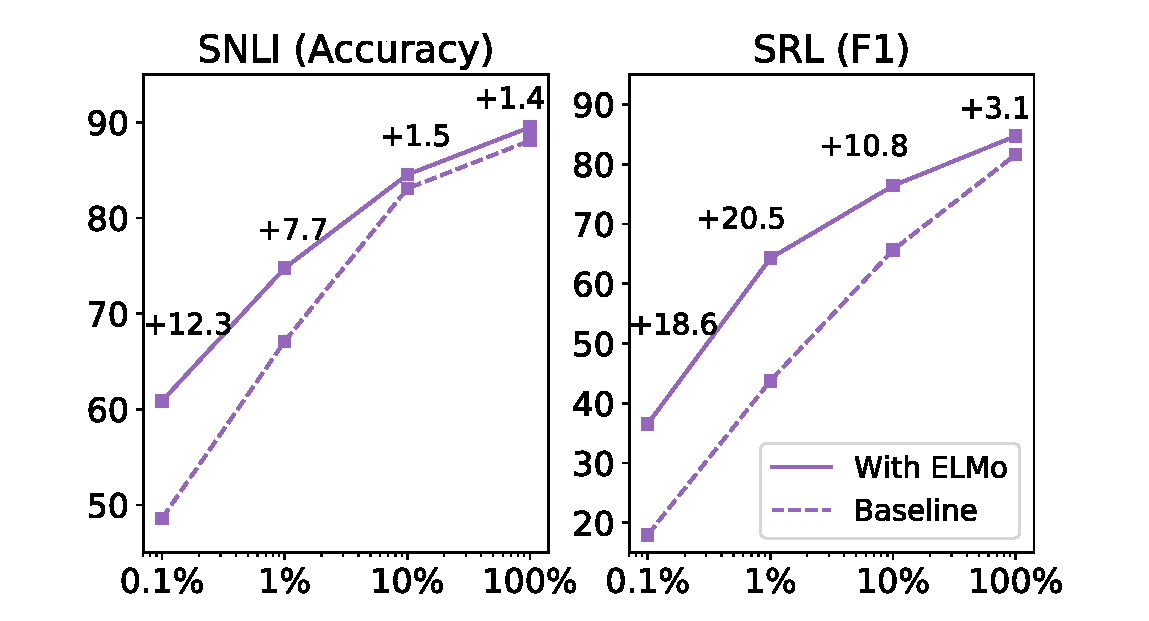
\includegraphics[width=0.48\textwidth]{elmo_training_set_size}
  \caption{Comparison of baseline vs. \ELMO{} performance for SNLI and SRL as the training set size is varied from 0.1\% to 100\%.
}
\end{figure}

\begin{figure}
  \label{fig:weight_visualization}
  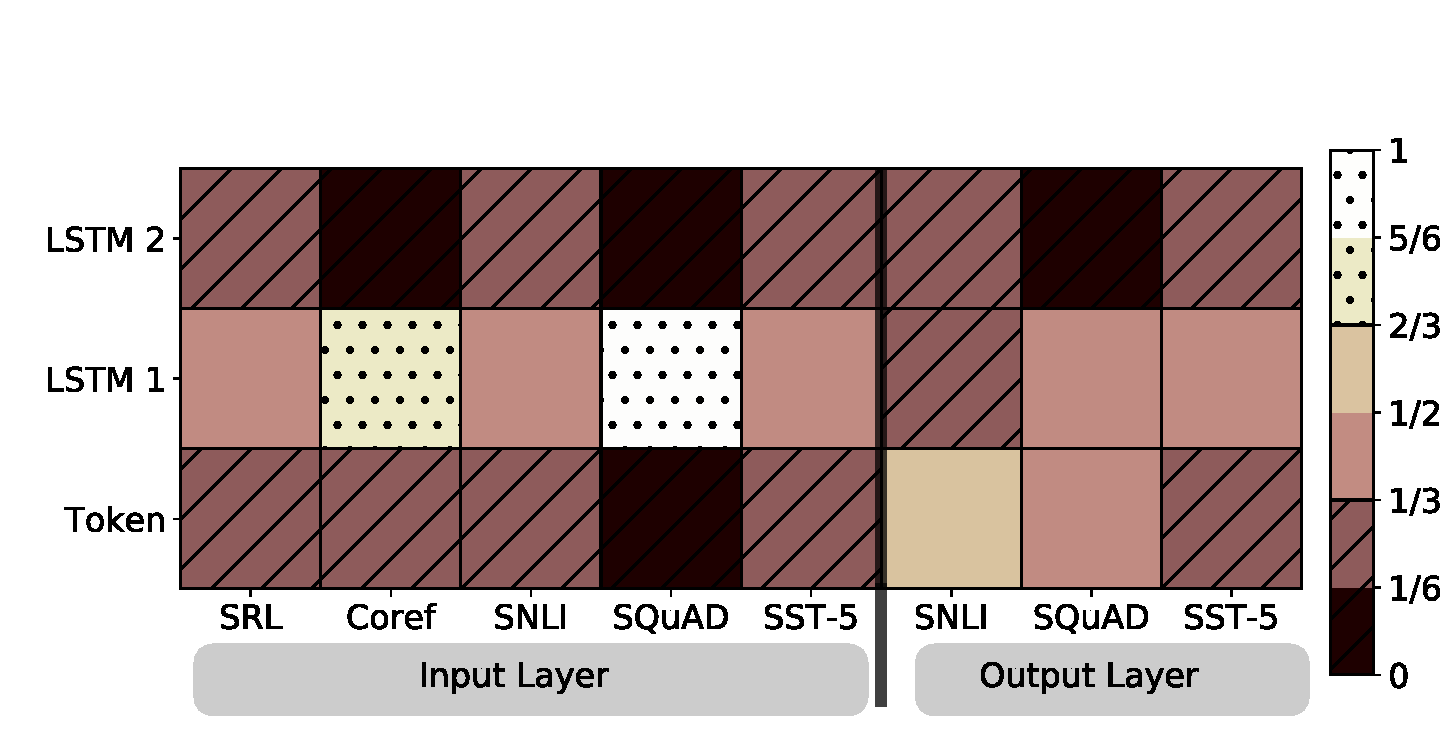
\includegraphics[width=0.48\textwidth]{weight_visualization}
  \caption{Visualization of softmax normalized biLM layer weights across tasks and \ELMO{} locations.  Normalized weights less then $1/3$ are hatched with horizontal lines and those greater then $2/3$ are speckled.
  }
\end{figure}




%%%%%%%%%%
\subsection{Sample efficiency}
\label{sec:sample_efficiency}
Adding \ELMO{} to a model increases the sample efficiency considerably, both in terms of number of parameter updates to reach state-of-the-art performance and the overall training set size. For example, the SRL model reaches a maximum development F$_1$ after 486 epochs of training without \ELMO.  After adding \ELMO, the model exceeds the baseline maximum at epoch 10, a 98\% relative decrease in the number of updates needed to reach the same level of performance.

In addition, \ELMO{}-enhanced models use smaller training sets more efficiently than models without \ELMO.
% for some reason \ref{fig:small_data} isn't working, so hard code the figure number...
Figure 1 compares the performance of baselines models with and without \ELMO{} as the percentage of the full training set is varied from 0.1\% to 100\%.
Improvements with \ELMO{} are largest for smaller training sets and significantly reduce the amount of training data needed to reach a given level of performance.
In the SRL case, the \ELMO{} model with 1\% of the training set has about the same F$_1$ as the baseline model with 10\% of the training set.


\subsection{Visualization of learned weights}
\label{sec:visualize_weights}
Figure 2 visualizes the softmax-normalized learned layer weights. %across the tasks.
%At the input layer, in all cases, the task model favors the first biLSTM layer, with the remaining emphasis split between the token layer and top biLSTM in task specific ways.
%For coreference and SQuAD, the first LSTM layer is strongly favored, but the distribution is less peaked for the other tasks.
At the input layer, the task model favors the first biLSTM layer.
For coreference and SQuAD, the this is strongly favored, but the distribution is less peaked for the other tasks.
%It is an interesting question for future work to understand why the first biLSTM layer is universally favored.
%the coreference and SQuAD models strongly preferring the first layer the remaining emphasis split between the token layer and top biLSTM, except for coreference and where it strongly favors the first biLSTM layer.
The output layer weights are relatively balanced, with a slight preference for the lower layers.
%In tasks benefit from including \ELMO{} at the output layers (SNLI, SQuAD and SST-5)\mgcomment{Awkward wording}, the output layer weights are relatively balanced, with a slight preference for the lower layers.

%\subsection{Importance of fine tuning on task data}

%\section{Conclusion and future work}  % ICLR
\section{Conclusion}  % NAACL
We have introduced a general approach for learning high-quality deep context-dependent representations from biLMs, and shown large improvements when applying \ELMO{} to a broad range of NLP tasks.
%Through ablations and other controlled experiments, we have also confirmed that the biLM represents different types of information at different layers, and that using all of them improves overall task performance.
Through ablations and other controlled experiments, we have also confirmed that the biLM layers efficiently encode different types of syntactic and semantic information about words-in-context, and that using all layers improves overall task performance.

%%%%%% ICLR
%Our approach raises several interesting questions for future work, broadly organized into two themes.

%\tinysection{``What is the best training regime for learning generally useful NLP representations?''}
%By choosing a biLM training objective, we benefit from nearly limitless unlabeled text and can immediately apply advances in language modeling, an active area of current research.
%However, it's possible that further decreases in LM perplexity will not translate to more transferable representations, and that other objective functions might be more suitable for learning general purpose representations.

%\tinysection{``What is the best way to use deep contextual representations for other tasks?''}
%Our method of using a weighted average of all layers from the biLM is simple and empirically successful.
%However, a deeper fusion of the biLM layers with a target NLP architecture may lead to further improvements. 
%%%%%%% END ICLR

\bibliography{deep_representations_bilm}
%\bibliographystyle{iclr2018_conference}
\bibliographystyle{acl_natbib}

%--ICLR
%\clearpage
%\section{Appendix}
%-- end ICLR


%%%%%%%%%%%%%%%%%%%%%%%%%%%%%%%%%%%%%%%%%%%%%%%%%%%%%%%%%%%%%%%%%%%%%%%%
% NAACL
\clearpage
\appendix
\setcounter{page}{1}
\section{Supplemental Material to accompany {\em Deep contextualized word representations}}

This supplement contains details of the model architectures, training routines and hyper-parameter choices for the state-of-the-art models in Section \ref{sec:results}.

All of the individual models share a common architecture in the lowest layers with a context independent token representation below several layers of stacked RNNs
-- LSTMs in every case except the SQuAD model that uses GRUs.

\subsection{Fine tuning biLM}
As noted in Sec. \ref{sec:pretrainedLMs}, fine tuning the biLM on task specific data typically resulted in significant drops in perplexity.
To fine tune on a given task, the supervised labels were temporarily ignored, the biLM fine tuned for one epoch
on the training split and evaluated on the development split.
Once fine tuned, the biLM weights were fixed during task training.

Table~\ref{table:lm_perplexities} lists the development set perplexities for the considered tasks.   In every case except CoNLL 2012, fine tuning results in a large improvement in perplexity, e.g., from 72.1 to 16.8 for SNLI.

The impact of fine tuning on supervised performance is task dependent.
In the case of SNLI, fine tuning the biLM increased development accuracy 0.6\% from 88.9\% to 89.5\% for our single best model.
However, for sentiment classification development set accuracy is approximately the same regardless whether a fine tuned biLM was used.

\subsection{Importance of $\gamma$ in Eqn. (1)}
The $\gamma$ parameter in Eqn. (\ref{eqn:weight_func}) was of practical importance to aid optimization, due to the different distributions between the biLM internal representations and the task specific representations.
It is especially important in the last-only case in Sec.~\ref{sec:alternate_weighting}.  
Without this parameter, the last-only case performed poorly (well below the baseline) for SNLI and training failed completely for SRL.


\subsection{Textual Entailment}
Our baseline SNLI model is the ESIM sequence model from \citet{Chen2017EnhancedLF}.
Following the original implementation, we used 300 dimensions for all LSTM and feed forward layers and pre-trained 300 dimensional GloVe embeddings that were fixed during training.
For regularization, we added 50\% variational dropout \citep{Gal2016ATG} to the input of each LSTM layer and 50\% dropout \citep{Srivastava2014DropoutAS} at the input to the final two fully connected layers.  All feed forward layers use ReLU activations.
Parameters were optimized using Adam \citep{Kingma2014AdamAM} with gradient norms clipped at 5.0 and initial learning rate 0.0004, decreasing by half each time accuracy on the development set did not increase in subsequent epochs.  The batch size was 32.

The best \ELMO{} configuration added \ELMO{} vectors to both the input and output of the lowest layer LSTM,
using (\ref{eqn:weight_func}) with layer normalization and $\lambda=0.001$.  Due to the increased number of parameters in the \ELMO{} model, we added $\ell^2$ regularization with regularization coefficient 0.0001 to
all recurrent and feed forward weight matrices and 50\% dropout after the attention layer.

Table~\ref{table:snli_test} compares test set accuracy of our system to previously published systems.
Overall, adding \ELMO{} to the ESIM model improved accuracy by 0.7\% establishing a new
single model state-of-the-art of 88.7\%, and a five member ensemble pushes the overall accuracy to 89.3\%.

%%%%%%%%%%%%%%%%%%%%%%%%%%%%%%%%%%%%%%%%%%%%%%%
% LM perplexities!
\begin{table}
\centering
\begin{tabular}{ll|l|l}
\multicolumn{2}{c|}{\textbf{Dataset}}           & \textbf{\begin{tabular}[c]{@{}l@{}}Before \\ tuning\end{tabular}} & \textbf{\begin{tabular}[c]{@{}l@{}}After\\ tuning\end{tabular}} \\  \hline \hline
\multicolumn{2}{l|}{SNLI}                        & 72.1            & 16.8                   \\ \hline
\multicolumn{2}{l|}{CoNLL 2012 (coref/SRL)}    & 92.3            & -                      \\ \hline
\multicolumn{2}{l|}{CoNLL 2003 (NER)}            & 103.2           & 46.3                  \\  \hline
\multirow{2}{*}{SQuAD}        & Context        & 99.1           & 43.5                  \\
                              & Questions     & 158.2          & 52.0                   \\ \hline
\multicolumn{2}{l|}{SST} & 131.5           & 78.6                                                           
\end{tabular}
\caption{Development set perplexity before and after fine tuning for one epoch on the training set for various datasets (lower is better).
Reported values are the average of the forward and backward perplexities.
}
\label{table:lm_perplexities}
\end{table}
%%%%%%%%%%%%%%%%%%%%%%%%%%%%%%%%%%%%%%%%%%%%%%%

%%%%%%%%%%%%%%%%%%%%%%%%%%%%%%%%%%%%%%%%
%%% SNLI TEST TABLE
\begin{table*}
\centering
\begin{tabular}{l|l}
\textbf{Model}                                                 & \textbf{Acc.} \\ \hline \hline
Feature based \citep{snliemnlp2015}                & 78.2                                                    \\
DIIN \citep{Gong2017NaturalLI}                      & 88.0                                                    \\
BCN+Char+CoVe \citep{McCann2017LearnedIT}       & 88.1                                                    \\
ESIM \citep{Chen2017EnhancedLF}                     & 88.0                                                    \\
ESIM+TreeLSTM \citep{Chen2017EnhancedLF} & 88.6                                                    \\
ESIM+\ELMO                                          & \textbf{88.7} $\pm$ 0.17                                           \\ \hline

DIIN ensemble \citep{Gong2017NaturalLI}             & 88.9                                                    \\
ESIM+\ELMO~ensemble                                 & \textbf{89.3}                                          
\end{tabular}
\caption{SNLI test set accuracy.\protect\footnotemark
Single model results occupy the portion, with ensemble results at the bottom.
}
\label{table:snli_test}
\end{table*}
%%%%%%%%%%%%%%%%%%%%%%%%%%%%%%%%%%%%%%%%


\subsection{Question Answering}
Our QA model is a simplified version of the model from \citet{ClarkAdvancingRC}. It embeds tokens by concatenating each token's case-sensitive 300 dimensional GloVe word vector \citep{Pennington2014GloveGV} with a character-derived embedding produced using a convolutional neural network followed by max-pooling on learned character embeddings. The token embeddings are passed through a shared bi-directional GRU, and then the bi-directional attention mechanism from BiDAF~\cite{Seo2016BidirectionalAF}. The augmented context vectors are then passed through a linear layer with ReLU activations, a residual self-attention layer that uses a GRU followed by the same attention mechanism applied context-to-context, and another linear layer with ReLU activations. Finally, the results are fed through linear layers to predict the start and end token of the answer. 

%%%%%%%%%%%%%%%%%%%% SQuAD TEST TABLE
\begin{table*}
\centering
\begin{tabular}{l|l|l}
\textbf{Model}                         & \textbf{EM}       & \textbf{F$_1$} \\ \hline \hline
BiDAF \citep{Seo2016BidirectionalAF}  & 68.0	& 77.3 \\
BiDAF + Self Attention  & 72.1	 & 81.1 \\
DCN+ & 75.1 &	83.1 \\
Reg-RaSoR  & 75.8 &	83.3 \\
FusionNet  & 76.0	 & 83.9 \\
r-net \citep{Wang2017GatedSN} & 76.5 &	84.3 \\
SAN \citep{liu2017stochastic} & 76.8 & 84.4 \\
BiDAF + Self Attention + \ELMO{} & \textbf{78.6}  & \textbf{85.8} \\ \hline
DCN+ Ensemble & 78.9 & 86.0 \\
FusionNet Ensemble & 79.0 & 86.0 \\
Interactive AoA Reader+ Ensemble & 79.1 & 86.5 \\
BiDAF + Self Attention + \ELMO{} Ensemble & \textbf{81.0}  & \textbf{87.4}

\end{tabular}
\caption{Test set results for SQuAD, showing both Exact Match (EM) and F$_1$.  The top half of the table contains single model results with ensembles at the bottom.
References provided where available.
}
\label{table:squad_test}
\end{table*}
%%%%%%%%%%%%%%%%%%%%%%%%%%%%%%%%%%%%%%%%

%%%%%%%%%%%%%%%%%%%% SRL TEST TABLE
\begin{table}
\centering
\begin{tabular}{l|l}
\textbf{Model}                                & \textbf{F$_1$} \\ \hline \hline
\citet{Pradhan2013TowardsRL}   & 77.5 \\
\citet{Zhou2015EndtoendLO}                & 81.3     \\
\citet{He2017DeepSR}, single                  & 81.7      \\
\citet{He2017DeepSR}, ensemble     & 83.4  \\ \hline
\citet{He2017DeepSR}, our impl. & 81.4         \\
\citet{He2017DeepSR} + \ELMO             & \textbf{84.6}       \\
\end{tabular}
\caption{SRL CoNLL 2012 test set F$_1$.
}
\label{table:srl_test}
\end{table}
%%%%%%%%%%%%%%%%%%%%%%%%%%%%%%%%%%%%%%%%


Variational dropout is used before the input to the GRUs and the linear layers at a rate of 0.2. 
A dimensionality of 90 is used for the GRUs, and 180 for the linear layers. We optimize the model using Adadelta with a batch size of 45. At test time we use an exponential moving average of the weights and limit the output span to be of at most size 17. We do not update the word vectors during training.

Performance was highest when adding \ELMO{} without layer normalization to both the input and output of the contextual GRU layer and leaving the \ELMO{} weights unregularized ($\lambda=0$).

Table \ref{table:squad_test} compares test set results from the SQuAD leaderboard as of November 17, 2017 when we submitted our system.
Overall, our submission had the highest single model and ensemble results, improving the previous single model result (SAN) by 1.4\% F$_1$ and our baseline by 4.2\%.  A 11 member ensemble pushes F$_1$ to 87.4\%, 1.0\% increase over the previous ensemble best.

% the footnote for SNLI table, must appear on same page as table
\footnotetext{A comprehensive comparison can be found at \url{https://nlp.stanford.edu/projects/snli/}}



\subsection{Semantic Role Labeling}
Our baseline SRL model is an exact reimplementation of \citep{He2017DeepSR}. Words are represented using a concatenation of 100 dimensional vector representations, initialized using GloVe \citep{Pennington2014GloveGV} and a binary, per-word predicate feature, represented using an 100 dimensional embedding. This 200 dimensional token representation is then passed through an 8 layer ``interleaved'' biLSTM with a 300 dimensional hidden size, in which the directions of the LSTM layers alternate per layer. This deep LSTM uses Highway connections \citep{Srivastava2015TrainingVD} between layers and variational recurrent dropout \citep{Gal2016ATG}. This deep representation is then projected using a final dense layer followed by a softmax activation to form a distribution over all possible tags. Labels consist of semantic roles from PropBank \citep{Palmer2005propbank} augmented with a BIO labeling scheme to represent argument spans. During training, we minimize the negative log likelihood of the tag sequence using Adadelta with a learning rate of 1.0 and $\rho = 0.95$ \citep{Zeiler2012ADADELTAAA}. At test time, we perform Viterbi decoding to enforce valid spans using BIO constraints. Variational dropout of 10\% is added to all LSTM hidden layers. Gradients are clipped if their value exceeds 1.0. Models are trained for 500 epochs or until validation F1 does not improve for 200 epochs, whichever is sooner. The pretrained GloVe vectors are fine-tuned during training. The final dense layer and all cells of all LSTMs are initialized to be orthogonal. The forget gate bias is initialized to 1 for all LSTMs, with all other gates initialized to 0, as per \citep{Jzefowicz2015AnEE}.

Table \ref{table:srl_test} compares test set F1 scores of our \ELMO{} augmented implementation of \citep{He2017DeepSR} with previous results. Our single model score of 84.6 F1 represents a new state-of-the-art result on the CONLL 2012 Semantic Role Labeling task, surpassing the previous single model result by 2.9 F1 and a 5-model ensemble by 1.2 F1.



\subsection{Coreference resolution}
Our baseline coreference model is the end-to-end neural model from \citet{Lee2017EndtoendNC} with all hyperparameters exactly following the original implementation.

The best configuration added \ELMO{} to the input of the lowest layer biLSTM and weighted the biLM layers using (\ref{eqn:weight_func}) without any regularization ($\lambda=0$) or layer normalization.
50\% dropout was added to the \ELMO{} representations.

Table \ref{table:coref} compares our results with previously published results.  Overall, we improve the single model state-of-the-art by 3.2\% average F$_1$, and our single model result improves the previous ensemble best by 1.6\% F$_1$.  Adding \ELMO{} to the output from the biLSTM in addition to the biLSTM input reduced F$_1$ by approximately 0.7\% (not shown).



%%%%%%%%%%%%%%%%%%%% COREF TEST TABLE
\begin{table}
\centering
\begin{tabular}{l|l}
\textbf{Model}                                & \textbf{Average F$_1$} \\ \hline \hline
\citet{Durrett2013EasyVA}   & 60.3 \\
\citet{Wiseman2016LearningGF}                & 64.2     \\
\citet{Clark2016DeepRL}                  & 65.7      \\
\citet{Lee2017EndtoendNC} (single) & 67.2         \\
\citet{Lee2017EndtoendNC} (ensemble) & 68.8         \\
\citet{Lee2017EndtoendNC} + \ELMO             & \textbf{70.4}       \\
\end{tabular}
\caption{Coreference resolution average F$_1$ on the test set from the CoNLL 2012 shared task.
}
\label{table:coref}
\end{table}
%%%%%%%%%%%%%%%%%%%%%%%%%%%%%%%%%%%%%%%%


\subsection{Named Entity Recognition}
Our baseline NER model concatenates 50 dimensional pre-trained Senna vectors \citep{NLPfromScratch:Collobert2011} with a CNN character based representation.  The character representation uses 16 dimensional character embeddings and 128 convolutional filters of width three characters, a ReLU activation and by max pooling.  The token representation is passed through two biLSTM layers, the first with 200 hidden units and the second with 100 hidden units before a final dense layer and softmax layer.
During training, we use a CRF loss and at test time perform decoding using the Viterbi algorithm while ensuring that the output tag sequence is valid.

Variational dropout is added to the input of both biLSTM layers.
During training the gradients are rescaled if their $\ell^2$ norm exceeds 5.0 and parameters updated using Adam with constant learning rate of 0.001.
The pre-trained Senna embeddings are fine tuned during training.
We employ early stopping on the development set and report the averaged test set score across five runs with different random seeds.

\ELMO{} was added to the input of the lowest layer task biLSTM.
As the CoNLL 2003 NER data set is relatively small, we found the best performance by
constraining the trainable layer weights to be effectively constant by setting $\lambda=0.1$ with (\ref{eqn:weight_func}).

Table \ref{table:ner_test} compares test set F$_1$ scores of our \ELMO{} enhanced biLSTM-CRF tagger with previous results. 
Overall, the 92.22\% F$_1$ from our system establishes a new state-of-the-art.
When compared to \citet{Peters2017SemisupervisedST}, using representations from all layers of the biLM provides a modest improvement.



%%%%%%%%%%%%%%%%%%%% NER TEST TABLE
\begin{table}
\centering
\begin{tabular}{l|l}
\textbf{Model}                                & \textbf{F$_1$ $\pm$ std.} \\ \hline \hline
\citet{NLPfromScratch:Collobert2011}$^\clubsuit$ & 89.59 \\
\citet{lample-EtAl:2016:N16-1} & 90.94 \\
\citet{Ma2016EndtoendSL}                & 91.2     \\
\citet{chiu-nichols-2016}$^{\clubsuit,\diamondsuit}$         & 91.62 $\pm$ 0.33  \\
\citet{Peters2017SemisupervisedST}$^\diamondsuit$     & 91.93 $\pm$ 0.19   \\
biLSTM-CRF + \ELMO   & \textbf{92.22 $\pm$ 0.10}
\end{tabular}
\caption{Test set F$_1$ for CoNLL 2003 NER task.
Models with $^\clubsuit$ included gazetteers and those with $^\diamondsuit$ used both the train and development splits for training.
}
\label{table:ner_test}
\end{table}
%%%%%%%%%%%%%%%%%%%%%%%%%%%%%%%%%%%%%%%%



\subsection{Sentiment classification}
We use almost the same biattention classification network architecture described in \citet{McCann2017LearnedIT}, with the exception of replacing the final maxout network with a simpler feedforward network composed of two ReLu layers with dropout. A BCN model with a batch-normalized maxout network reached significantly lower validation accuracies in our experiments, although there may be discrepancies between our implementation and that of \citet{McCann2017LearnedIT}. To match the CoVe training setup, we only train on phrases that contain four or more tokens. We use 300-d hidden states for the biLSTM and optimize the model parameters with Adam~\cite{Kingma2014AdamAM} using a learning rate of 0.0001. The trainable biLM layer weights are regularized by $\lambda=0.001$, and we add ELMo to both the input and output of the biLSTM; the output ELMo vectors are computed with a second biLSTM and concatenated to the input. 

%%%%%%%%%%%%%%%%%%%% SST TEST TABLE
\begin{table}
\centering
\begin{tabular}{l|l}
\textbf{Model}                                & \textbf{Acc.} \\ \hline \hline
DMN \citep{kumar2015ask} & 52.1 \\
LSTM-CNN \citep{zhou2016text} & 52.4 \\
NTI \citep{munkhdalaineural} & 53.1 \\
BCN+Char+CoVe \citep{McCann2017LearnedIT} & 53.7 \\
BCN+\ELMO   & \textbf{54.7}
\end{tabular}
\caption{Test set accuracy for SST-5.
}
\label{table:sst_test}
\end{table}
%%%%%%%%%%%%%%%%%%%%%%%%%%%%%%%%%%%%%%%%



\end{document}
